\section{Discussion}
The diagnostic experiments conducted in this study reveal a fundamental tension in machine learning approaches to remote sensing hydrology: the tradeoff between local spatial accuracy and generalizable physical process representation.

\subsection{Scope Limitations of the Spatial Baseline Model}
While the Combined Random Forest model achieves the highest out-of-distribution $F_1$-score performance on our test set, it exhibits significant scope limitations when used as a generalizable hydrological model. We emphasize that the high feature importance for terrain features reflects a statistical association within our predictive benchmark rather than a direct physical cause of inundation. Topography acts as a structural container that influences where water can physically accumulate and route, but the physical activation of these pathways is driven by meteorological and hydraulic gradients. Unlike differentiable physical models (e.g., \citealp{Feng2023The}) that represent energy and mass conservation, Random Forest learns statistical relationships associated with terrain features without representing the underlying hydraulic controls, floodplain connectivity, or soil water storage dynamics. The applicability of Random Forest is constrained by several factors:
\begin{enumerate}
    \item \textbf{Reduced Spatial Transferability:} Random Forest models are vulnerable to reduced transferability when terrain configurations differ from the training region. Because these models partition feature space based on local geographic attributes (such as elevation and distance-to-river coordinates), they struggle to extrapolate when transferred to regions with distinct terrain features, leading to spatial extrapolation errors. This spatial overfitting restricts the model's capacity to represent floodplain connectivity in adjacent sub-basins.
    \item \textbf{Lack of Temporal Catchment Memory:} Empirical baselines lack an explicit representation of temporal state transitions or mass-balance conservation. In the Indus Delta, soil moisture memory and groundwater storage dynamics act as temporal buffers that sustain wetlands and vegetation during dry-down periods. This extends the work of \citet{Kratzert2018} and \citet{Nearing2020What}, who demonstrated that recurrent neural architectures like LSTMs succeed in rainfall-runoff modeling by implicitly tracking these storage states. However, in low-relief floodplains, the absence of an explicit physical routing and storage state in Random Forests prevents the model from capturing the delay between catchment-scale recharge and localized wetland inundation, which is crucial for evaluating residence times and surface-subsurface exchange.
    \item \textbf{Inability to Represent Latent Hydrological States:} The baseline model directly maps static inputs to occurrence outputs. Rather than representing physical causal drivers, it estimates empirical probabilities of water presence. It does not learn physically consistent state variables such as Terrestrial Water Storage, Topological Connectivity, or Tidal Pressure Head, which are vital for water resource management and are typically represented in process-based formulations (e.g., \citealp{Feng2023The}).
    \item \textbf{Inability to Model Delayed Routing:} Random Forest treats each monthly observation as independent, failing to represent geomorphological and hydraulic routing delays. Our findings regarding the multi-month routing delay in coastal wetlands are consistent with the long-term storage and regulatory delays characterized globally by \citet{Scanlon2023Global}. Without dynamic routing, empirical models cannot resolve how upstream floodwaves activate localized floodplain connectivity or how coastal backwater effects alter residence times in tidal wetlands.
\end{enumerate}

Furthermore, the bootstrap confidence intervals reported for our ablation study comparing the Terrain-only and Combined models exhibit substantial overlap. This statistical overlap implies that the slight numerical difference obtained by incorporating dynamic meteorological forcing is indistinguishable from random sampling variance. Coupled with the non-significant McNemar test, these intervals suggest that terrain features represent the primary spatial control on surface water boundaries in our predictive configuration, and that dynamic climate inputs do not provide statistically detectable spatial boundary information. The overlapping confidence intervals serve as a quantitative indicator of spatial boundary stability: under the evaluated forcing resolution, the spatial delineation of flood boundaries is so strongly constrained by local geomorphology that the addition of meteorological forcing does not alter the predicted boundary geometries in a statistically robust manner.

\subsection{Hydrological Process Interpretation: Connectivity, Storage, and Routing Lags}
The dominance of terrain features over climate variables in our predictive models reflects key physical mechanisms of floodplain connectivity and water storage in low-relief coastal systems. Topography acts as a first-order structural constraint on connectivity in the Indus Delta, which is characterized by an extremely flat gradient (typically less than 1:10,000 slope). In such environments, gravity-driven routing is shaped by minor micro-topographical depressions, paleochannels, and artificial structures (such as embankments, levees, and barrages). Geomorphic connectivity in this low-relief system is defined by topological pathways and sub-grid channel networks that dictate where water can physically flow and pool. When floodwaters spill over banks, these micro-topographic features act as localized floodplain storage zones, retaining large volumes of water and delaying drainage. Local elevation ($z$), distance to the nearest river channel ($D_{\text{river}}$), and distance to the coastline ($D_{\text{coast}}$) define these topographic storage containers. Consequently, the high statistical feature importance of terrain features reflects the physical reality that the boundaries of inundation are structurally constrained by these geomorphological containers, defining the spatial extent where water can physically accumulate. This flat topography and high floodplain storage capacity reduce flow velocities, extending the hydrological residence time of surface water in the delta compared to steep catchments, where dynamic channel hydraulics and high-frequency runoff velocities modulate the spatial flood wave propagation.

While geomorphology controls the spatial boundaries, the dynamic timing of inundation is modulated by temporal routing and storage-recharge mechanisms.

The observed three-month lag is consistent with a delayed routing response in a managed delta system influenced by reservoirs, barrages, and channel storage. However, this should be interpreted as a statistical routing signal rather than proof of a single physical mechanism, because discharge, tidal stage, and groundwater observations are not available in this study.

Main-channel routing velocities are significantly altered by the sequential regulation of major barrages (including Sukkur and Kotri), which control flow distributions for canal networks and environmental releases. The Indus basin features some of the largest reservoirs (e.g., Tarbela and Mangla) and barrages in the world, which operate to buffer monsoonal precipitation and release water systematically over months. This regulation introduces a massive catchment memory. Our findings regarding the multi-month routing delay in coastal wetlands are consistent with the long-term storage and regulatory delays characterized globally by \citet{Scanlon2023Global}, where large-scale reservoir operations and regional groundwater storage recharge/depletion delays decouple local precipitation from downstream wetness. Upstream monsoonal rainfall is stored in reservoirs and routed through thousands of kilometers of channels and barrages (including the Kotri Barrage just upstream of the delta), reaching the coastal wetlands as delayed environmental flows or discharge events months later.

Furthermore, this routing delay interacts with local hydraulic controls and tidal propagation in the coastal zone. In coastal wetlands, upstream freshwater routing meets marine tidal pressure heads. Tides propagate daily through the dense creek network, creating a backwater effect that propagates up to 80 km inland. This tidal pressure head slows down channel flow velocities, raising local water levels, obstructing freshwater drainage, and extending the residence time of water in the deltaic floodplains. Without explicit representation of these hydraulic controls, empirical models are unable to resolve the physical mechanisms behind this routing delay, illustrating the limits of purely statistical associations.

In contrast, the negative correlation observed between precipitation and surface wetness in irrigated croplands indicates a human-induced decoupling of local soil moisture and inundation from natural climate drivers. In the Indus Delta, canal irrigation networks divert upstream river discharge during the dry season to sustain agricultural activities. This artificial water routing activates geomorphological flow paths (irrigation canals, fields) during dry periods when local rainfall is zero. The irrigation timing is strictly governed by the agricultural cropping calendar, specifically the dry-season Rabi (winter) and monsoonal Kharif (summer) crops, which releases water out-of-phase with local precipitation. This anthropogenic management creates an out-of-phase relationship between rainfall and surface wetness. In comparison, in natural systems without canal regulation, soil moisture and wetland boundaries typically expand in phase with local precipitation. The negative rainfall–wetness relationship in croplands should be interpreted cautiously because irrigation releases, crop phenology, and SAR backscatter sensitivity may all contribute to the observed pattern.

In contrast to unregulated catchments where empirical architectures like LSTMs succeed in capturing temporal memory by implicitly tracking soil water storage and routing states \citep{Kratzert2018, Nearing2020What}, our results indicate that in heavily managed deltaic systems, the lack of explicit physical routing and human-induced storage states (such as reservoir operations and canal diversions) prevents these models from generalizing, as the physical links between climate drivers and surface inundation are structurally altered by anthropogenic hydraulic controls. Thus, the observed spatial-temporal patterns are not merely statistical artifacts but represent the physical signature of a highly regulated geomorphological system.

\subsection{Future Research Directions: Motivating Physically Constrained State-Space Models}
The representation collapse of sequence models during dry periods and the spatial transferability limits of Random Forest highlight the need to move beyond purely empirical architectures. These findings motivate the future development of physically constrained state-space models, such as a Physics-Constrained Hydrological State-Space Model (PHSSM) conceptually outlined in Supplementary Note~S1, as a promising research pathway. Such models would conceptually integrate temporal mass-balance concepts with spatial terrain boundary constraints to separate the dynamic timing of inundation from its static boundaries, without relying on purely statistical mappings. While such frameworks represent conceptual directions, their future implementation will need to address the challenges of parameter equifinality under coarse forcing, potentially by integrating catchment-scale physical observations (e.g., river discharge records) to constrain latent water storage variables.

\begin{figure}[t]
\centering
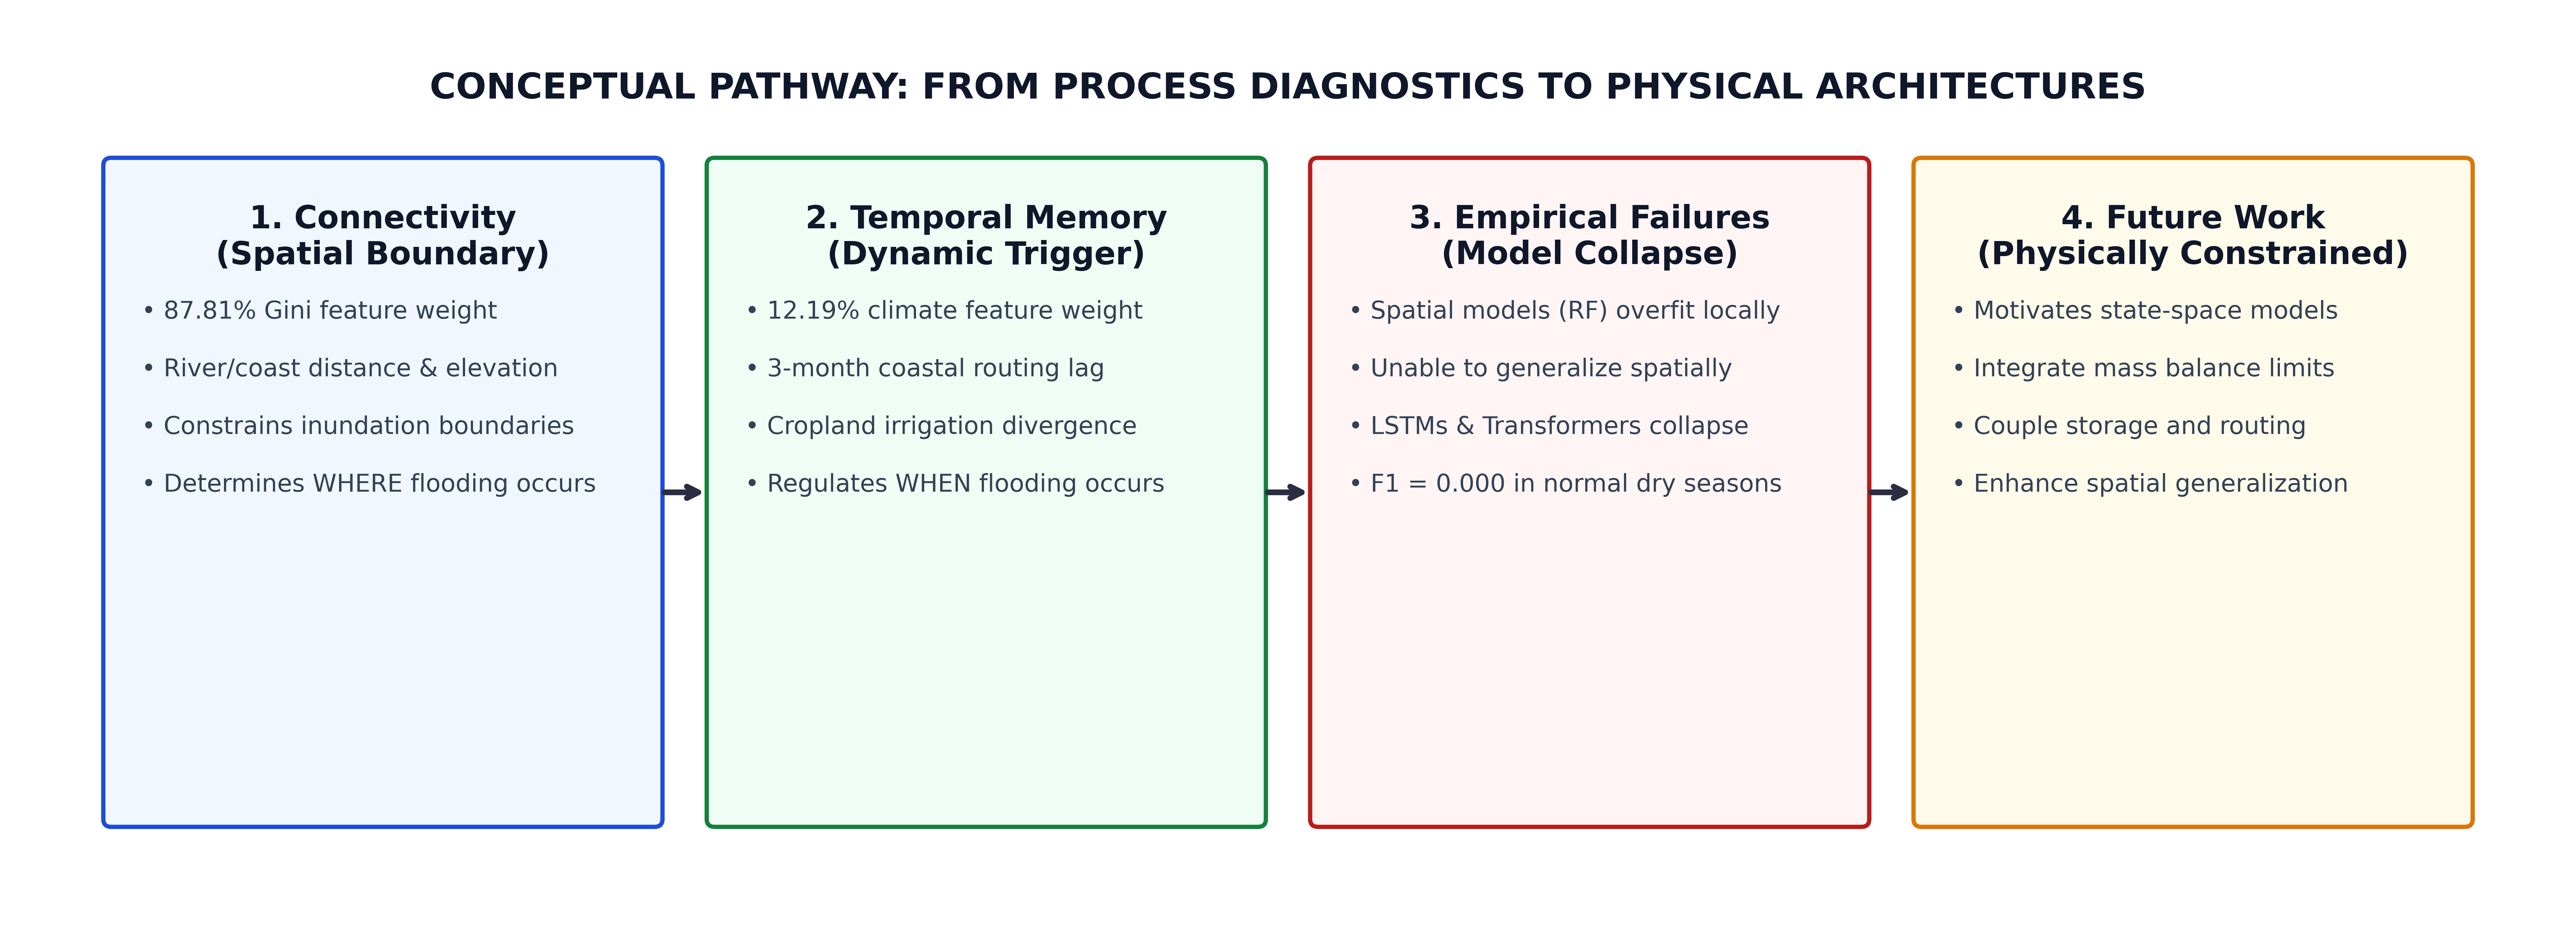
\includegraphics[width=1.0\linewidth]{figures/fig7_motivation.png}
\caption{Conceptual pathway mapping the findings of this study to future model designs: (1) static topographic connectivity shapes the spatial boundaries; (2) dynamic meteorology activates temporal inundation over lags; (3) purely empirical models fail via spatial overfitting or temporal collapse; and (4) these findings motivate physically constrained state-space models as a promising future direction.}
\label{fig:motivation_pathway}
\end{figure}

\subsection{Threats to Validity}
Several limitations and uncertainties in our benchmark study must be acknowledged, which affect the interpretation of our findings:
\begin{enumerate}
    \item \textbf{Uncertainty in Sentinel-1 Thresholding and Crop Phenology:} The target inundation label was derived using a static backscatter threshold ($VV < -15\text{ dB}$). Wind-induced surface roughness, emergent canopy closure, and soil salinity variations introduce sub-pixel classification errors. In agricultural fields, crop growth cycles alter canopy structure and vegetation water content, mimicking or masking water signatures. Consequently, the negative correlation ($r = -0.299$) in croplands could partly reflect crop canopy changes rather than true surface wetness, complicating interpretation in farmed zones. Future work should incorporate a backscatter intensity histogram to visually illustrate class separability under varying moisture conditions.
    \item \textbf{Absence of Streamflow and Discharge Observations:} The study lacks continuous river discharge records at the Kotri Barrage (the delta's primary inlet). Without upstream discharge inputs, the model cannot distinguish between upstream reservoir releases and local runoff events, preventing physical mass-balance validation and introducing uncertainty in routing lag timing.
    \item \textbf{Absence of Coastal Tidal Gauge Observations:} The model does not include tidal stage observations, despite the delta's proximity to the sea. Tides introduce oceanic pressure heads and backwater effects that delay floodplain drainage and extend residence times. Omitting tidal stage variables prevents separating tidal backwater delays from riverine routing lags, limiting our ability to verify the mechanisms behind the 3-month coastal wetland lag.
    \item \textbf{Absence of Groundwater Observations:} Continuous piezometric head observations were unavailable. In the Indus Delta, shallow aquifers recharge during high flows and sustain surface wetlands through capillary rise during dry-downs. Lacking groundwater table data prevents direct validation of subsurface infiltration and return-flow dynamics.
    \item \textbf{Spatial Resolution Mismatch of Climate Forcing:} CHIRPS precipitation ($\sim$5\,km) and ERA5-Land variables ($\sim$9\,km) are coarse relative to the Indus Delta channel network ($<$30\,m). Coarse forcing cannot resolve sub-grid channel wetting or localized irrigation, which is the primary cause of sequence model representation collapse ($F_1$-score $= 0.000$ without coordinates), as adjacent pixels receive identical meteorological inputs.
    \item \textbf{Single-Basin Study Focus:} All experiments were conducted within the Indus River Delta. Because the Indus is an extremely regulated and arid deltaic basin, this single-basin focus restricts the external validity of our findings, as geomorphological-dominance relationships may differ in humid, unregulated, or high-relief systems.
    \item \textbf{Model Transferability Limitations:} Random Forest models partition feature space based on local coordinates and terrain features. Because terrain configurations vary across basins, the models are vulnerable to spatial extrapolation errors, which restricts model transferability to adjacent sub-basins with distinct terrain features.
\end{enumerate}

\subsection{Spatial Resolution of Climate Forcing and Interpretation Caveat}
The observed dominance of terrain features over climate variables should be interpreted within the spatial resolution limits of the forcing datasets employed in this study. CHIRPS precipitation has a native resolution of approximately 5.5\,km and ERA5-Land of approximately 9\,km, while the Indus Delta channel network operates at spatial scales of 30\,m or finer. At these coarse meteorological resolutions, precipitation and evapotranspiration fields cannot resolve sub-pixel channel wetting, tidal backwater intrusion, or localized irrigation recharge gradients. Consequently, part of the observed low predictive contribution of climate variables may reflect a spatial scale mismatch between the input resolution and the target hydrological processes, rather than an intrinsic absence of climate influence at finer scales. Higher-resolution hydrometeorological products---such as sub-kilometer precipitation estimates or reanalysis downscaling---may capture additional dynamic variability not resolved by the forcing datasets used here, and future work should evaluate the sensitivity of these findings to input resolution.

\subsection{Scope of Inference and External Validity}
The findings in this study indicate that terrain features account for most of the predictive feature importance in surface water occurrence among the tested predictors. However, we emphasize that these conclusions are primarily valid for low-relief coastal systems, tidal deltas, and highly regulated floodplains. In mountainous basins or steep temperate river networks, dynamic channel hydraulics and high-frequency runoff peaks play a much more active role in defining spatial flood boundaries. Consequently, the decoupling of spatial geomorphological constraints from temporal climate triggers observed here should be carefully re-evaluated when applied to systems with complex hydraulic gradients.

\subsection{Practical Implications}
These findings are relevant for flood forecasting, reservoir management, irrigation planning, wetland monitoring, and delta resilience. The results suggest that static terrain features provide a strong constraint on where surface water can appear, while climate forcing acts mainly as a timing signal. This is useful for hydrological model design because it shows that coarse meteorological data alone may be insufficient to resolve delta-scale flood boundaries. The findings also support future physics-based models that combine storage, routing, and geomorphological connectivity in a single framework.

\begin{table}[t]
\caption{Summary of core scientific findings, empirical evidence, statistical validation, and corresponding manuscript contributions.}
\label{tab:contribution_summary}
\centering
\small
\begin{tabular}{p{2.8cm} p{2.8cm} p{4.0cm} p{2.8cm}}
\hline
\textbf{Finding} & \textbf{Evidence} & \textbf{Statistical Support} & \textbf{Paper Contribution} \\
\hline
Geomorphological Control & 87.81\% Gini feature importance in Random Forest & McNemar test yields $p = 0.2584$ comparing Terrain-only and Combined models & Topographic control over spatial boundaries (noting statistical power limits for small differences) \\
\hline
Hydrological Memory & 3-month precipitation routing lag in coastal wetlands & Temporal cross-correlation analysis & Routing lag and cropland correlation analysis \\
\hline
Sequence Model Collapse & F1 = 0.000 during normal dry periods for LSTM and Transformer & Diagnostic threshold sweeps and class imbalance testing & Sub-pixel channel smoothing limits sequence models \\
\hline
\end{tabular}
\end{table}

